\subsection{Network Baselining: Measured vs Relative}
First, this paper makes a distinction between a Measured Network Baseline and a Relative Network Baseline.  A Measured Network Baseline is a ``true'' baseline in a traditional sense, as a series of objective measurements on the performance and behavior of a computer network \cite{cisco_2017}, ideally conducted prior to the moment users begin to utilize the network in order to properly capture the autonomic events and activities occurring on the network by simply existing (vulnerability scans, DNS resolution queries, load balancing, etc.) \cite{1212675}. It is from this baseline that network security professionals attempt to filter out the every day workings of a network from the anomalous behaviors which they hope to detect. However many extant networks have not been baselined, and more importantly change over time. The approach in this paper is to introduce the concept of a Relative Network Baseline by identifying means and methods to which conduct baseline measurements on existing operating networks by recording network traffic, extrapolating and describing ``normal'' behaviors with machine learning and statistical methods, and create models of this behavior.

We do acknowledge certain challenges and assumptions in this approach. Accuracy of any baseline on a preexisting network could naturally be impeded by several factors: incomplete accounting of network devices, the presence of an adversary or Advanced Persistent Threat (APT) on the network, a lack of representative data due to volume or time, as well as benign abnormal host activity.  However, even with the drawbacks of a performing a relative baseline, it is our position that valuable insights can still be achieved.

\subsection{Dataset}
The body of this work was conducted in the Lincoln Research Network Operations Center (LRNOC) within MIT Lincoln Laboratory, having access to over five years of network flow data upon which to conduct analysis. Metadata was collected through a RESTful API to the network traffic and flow records and aggregated at 30 second intervals. The standard network five-tuple was collected in addition to two more features available by virtue of the aggregation:

\begin{table}[htbp]
\centering
\caption{Dataset Features}
\label{tab:dataset}
\begin{tabular}{|c|c|c|c|c|c|c|}
\hline
\multirow{2}{*}{Time} & \multicolumn{2}{c|}{IP} & \multicolumn{2}{c|}{Port} & \multicolumn{2}{c|}{Aggregated} \\ \cline{2-7} 
 & Src & Dst & Src & Dst & Payload & Packets \\ \hline
\end{tabular}
\end{table}

The aggregated process yields the total payload size (in bytes) as well as the number of packets transferred between unique IP and Port pairs within the user-selected interval size (in this case, 30 seconds). For the purposes of this paper, we further loosely define ``sessions'' as unique, directional flows within the user-selected time interval.

\subsection{Exploration Activity}

\begin{figure*}
	\centering
	\begin{subfigure}{9cm}
	\centering
	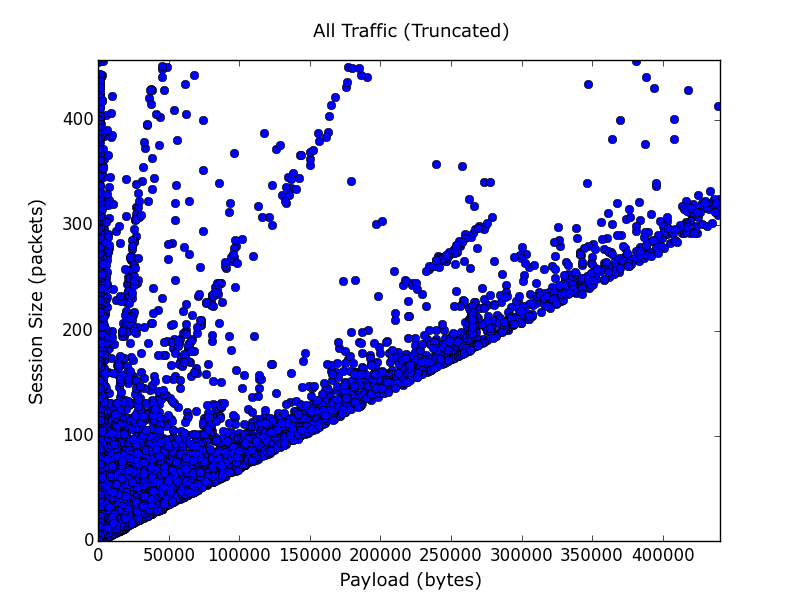
\includegraphics[width=\linewidth]{paperplots/everything.png}
	\label{subfig:all_traffic}
	\caption{Linear clustering within the dataset (zoomed)}
	\end{subfigure}%
	\begin{subfigure}{9cm}
	\centering
	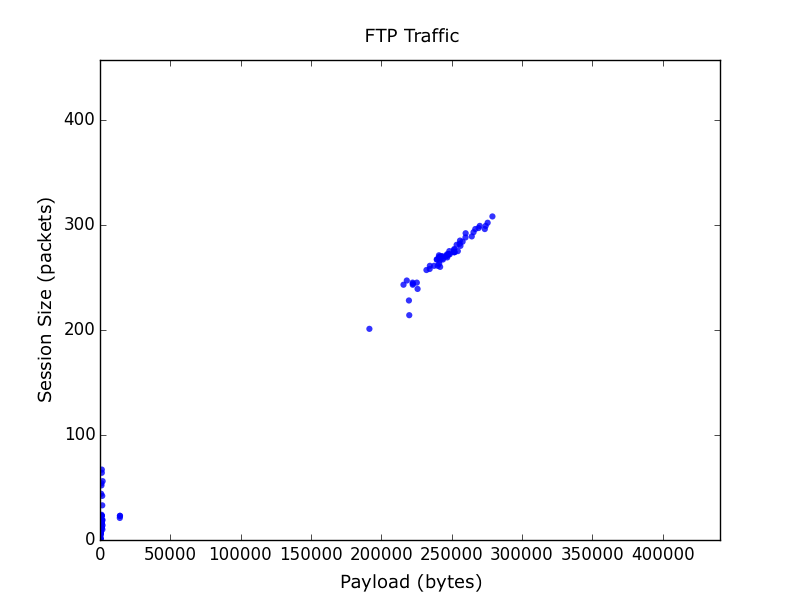
\includegraphics[width=\linewidth]{paperplots/ftp.png}
	\label{subfig:ftp}
	\caption{Manually verified cluster of FTP traffic, isolated from Sub. (a)}
	\end{subfigure}
	\caption{Exploration activity using manual analysis methods}
	\label{fig:explore}
\end{figure*}


Our efforts consider the linear relationship between the number of packets transmitted in a single session versus the amount of data passed within the payload (or content) of the communication. In this sense, one should be able to ultimately differentiate such traffic patterns as scanning activities (high packet counts/low data) from download or upload activity (minimized packets/maximized data).

Broadly speaking, structure became immediately apparent (as seen in Figure \ref{fig:explore}) where the traffic displayed linear behaviors, prompting this analysis. The first observation to note is the hard limit line -- an intrinsic network behavior related the the maximum transmission unit (MTU), effectively plotting the minimum number of packets necessary to convey the largest amount of data. The second characteristic of note is the linear clusters seemingly radial from the point of origin -- the very characteristic in which this analysis attempts to classify.

Manual analysis revealed that the cluster depicted in Subfigure (a) was FTP traffic, as seen in Subfigure (b), confirming the hypothesis that at least some traffic behaved linearly and served enough evidence to warrant our investigation. Also of note is the small cluster of traffic near origin of Subfigure (b) consisting of the server response traffic, highlighting the difference between inbound and outbound network traffic.